\documentclass[11pt, a4paper, english, twoside, notitlepage, openright]{report}

\usepackage[a4paper, total={15cm, 22cm}]{geometry}
\usepackage{iipr}
\fancyhead[RO, LE]{ }
\fancyhead[LO]{\nouppercase \leftmark}	% Heading on odd pages: Chapter name on the left
\fancyhead[RE]{\nouppercase \rightmark} % Heading on even pages: Section on the right
\fancyfoot[LE,RO]{\thepage} % Roman numbering, foot left on even, foot right on odd pages
\fancyfoot[CE]{Doble Grado en Matem\'aticas e Ingenier\'ia Inform\'atica} %Foot: Center, even pages
\fancyfoot[CO]{Universidad Complutense de Madrid (UCM)} %Foot: Center, odd pages
\renewcommand{\footrulewidth}{0.4pt} % Rule on top of foot
\renewcommand{\headrulewidth}{0.4pt} % Rule below headings
\pagestyle{fancy}

\usepackage{tikz}
\usetikzlibrary{calc}

\begin{document}

\pagenumbering{roman}
\begin{titlepage}

\title{\huge{\textsc{Complexity Analysis of\\
Polynomial Algorithms}} \\
\protect
\includegraphics[scale=0.2]{ucm.pdf}}
\author{Ignacio Iker Prado Rujas \\
Universidad Complutense de Madrid (UCM) \\
Doble Grado en Matem\'aticas e Ingenier\'ia Inform\'atica}
\date{\today}
\maketitle
\thispagestyle{empty}

\begin{center}
Tutors: \\
Juan Ram\'on Delgado, Jos\'e F. Fernando \textit{\&} Jos\'e M. Gamboa \\
\
\end{center}

%\newpage	
%\thispagestyle{empty}
\begin{abstract} This work is about different proofs of the same fact and a computational comparison between them, looking for the most efficient one.

Let $R$ be a real closed field and $n\geq 2$. Then: 
	
(1) For every finite subset $F$ of $R^n$, the semialgebraic set $R^n\setminus F$ is a polynomial image of $R^n$. 
	
(2) Given independent linear forms $h_1,\dots,h_r$ of $R^n$, the semialgebraic set $\{h_1>0,\dots,h_r>0\}\subset R^n$ is a polynomial image of $R^n$.
	
The key result here is that $\Qu:=\{x>0,y>0\}$ is a polynomial image of $R^2$. This assert is proved in three different ways: a first approach using some basic results in real algebraic geometry as Sturm's theorem and the Curve Selection Lemma and the aid of a computer; a second and shorter one, using the composition of three rather simple polynomial maps; and a third one that applies arguments of algebraic topology, without the aid of computer computations.
	
	(...)
\end{abstract}

\end{titlepage}


\tableofcontents
\thispagestyle{empty}

\begin{chapter}{Polynomial images of $R^n$}
\pagenumbering{arabic}    % Numbering from 1

\begin{section}{Introduction}
\begin{definition}\label{polyMap} Let $R$ be a \hyperref[realCField]{real closed field} and $m,n\in\N_{>0}$. A map $f:=(f_1,\dots,f_n):R^m\to R^n$ is said to be \em polynomial \em if $f_i\in R[x_1,\dots,x_m]$ for $i=1,\dots,n$. 
\end{definition}
	
A very famous theorem by Tarski and Seidenberg states the following:
\begin{theorem}[\em Tarski-Seidenberg\em]\label{tarskiSeidenberg} \em The image of every polynomial map $f: R^m \longrightarrow R^n$ is a \hyperref[semialgSet]{semialgebraic subset} of $R^n$. \em
\end{theorem}
	
In this work we study a sort of converse of this statement. In an \emph{Oberwolfach} week, J.M. Gamboa \cite{g} proposed to characterize the semialgebraic subsets of $R^n$ that are polynomial images of some $R^m$. Particularly interesting seems to be the study of those open semialgebraic subsets of $R^n$ that are polynomial images of $R^n$, because this is related with the real jacobian conjecture.
	
\begin{notation} We need to mention to which topology we refer to when we talk about closures, boundaries, etc. More specifically, the \em exterior boundary \em of a subset $S\subset R^n$ is $\delta S:=\overline{S}\setminus S$, with $\overline{S}$ being the \em closure \em of $S$ in the usual topology of $R^n$. In addition we will denote by $\overline{S}^{\text{zar}}$ the closure of $S$ with respect to the \hyperref[zariski]{Zariski topology} of $R^n$. We will say that a semialgebraic subset $A\subset R^n$ is \em Zariski-irreducible \em if its Zariski closure $\overline{A}^{\text{zar}}$ is an irreducible algebraic set.
\end{notation}
	
\begin{subsection}{Necessary conditions and examples} To begin working on this idea, we provide some necessary conditions for a set $S\subset R^n$ to be a polynomial image of $R^m$. 
	
If $m=n=1$, that is, for a polynomial function $f:R\to R$, its image $f(R)$ is either a \em singleton, \em that is, a set with a unique point if the function $f$ is constant, or an unbounded closed interval, for example if $f(x)=x^2$, or $f(R)=R$ if $f$ is a polynomial of odd degree.
	
In the general case, by \hyperref[tarskiSeidenberg]{Tarski-Seidenberg}, $S$ must be a semialgebraic set and, as $R^n$ is semialgebraically connected, $S$ is semialgebraically connected too. Even more, by the identity principle for polynomials, $S$ is Zariski-irreducible and \hyperref[pureDim]{pure dimensional}.
	
	% Añadir el teorema de Shiota y la definición de Nash map? NO
	
But to be a polynomial image of some $R^m$ is a restrictive condition, and there are more constrains than those quoted above. 
	
\begin{definition} A polynomial map $f:R^m\to R^n$ is said to be \em semialgebraically proper at a point $p\in R^n$ \em if there exists an open neighbourhood $K$ of $p$ such that the restriction $f|_{f^{-1}(K)}:f^{-1}(K)\to K$ is a \hyperref[properMap]{semialgebraically proper map}.
\end{definition}
	
\begin{definition} A \em parametric semiline \em of $R^n$ is the image of $R$ under a non-constant polynomial map $R\to R^n$.
\end{definition}
	
It is clear that every parametric semiline is semialgebraically closed, since every polynomial map from $R$ to $R^n$ is semialgebraically proper. Let $\S_f$ denote the set of points $p\in R^n$ at which $f$ is \textbf{not} semialgebraically proper.
	
\begin{theorem}[\em Jelonek\em]\label{jelonek}\em Let $f:R^2\to R^2$ be a \hyperref[dominant]{dominant} polynomial map. Then $\S_f$ is a finite union of parametric semilines.\em
\end{theorem}
	
With these ideas in mind, we present in the following proposition some obstructions for a semialgebraic set to be a polynomial image of $R^n$. 
\begin{proposition}\label{propIntro} Let $f: R^m\to R^n$ be a polynomial map and $S:=f(R^m)$.
\begin{enumerate}[\em(1)\em]
\item $\delta S \subset\S_f$.
\begin{Proof} Suppose $p\in\delta S\setminus \S_f$. Since $p\notin\S_f$, there exists an open neighbourhood $K$ of $p$ such that the restriction $f|_{f^{-1}(K)}:f^{-1}(K)\to K$ of $f$ is proper. Thus its image $K\cap S$ is a closed subset of $K$. Hence, $p\in K\cap\overline{S}=K\cap(\overline{K\cap S})=K\cap S$, which yields in a contradiction.
\end{Proof}
\item Let $m=n=2$ and $\Gamma$ be a $1$-dimensional irreducible component of $\overline{\delta S}^{\text{zar}}$. Then $\Gamma$ is the Zariski closure of a parametric semiline of $R^2$.
\begin{Proof} As $f$ is a dominant map, it follows from Theorem \ref{jelonek} that $\S_f$ is a finite union of parametric semilines, say $M_1,\dots, M_s$ in $R^2$. Then, using (1) we get: $\Gamma\subset\overline{\delta S}^{\text{zar}}\subset \overline{\S_f}^{\text{zar}}=\bigcup_{i=1}^s\overline{M_i}^{\text{zar}}$. Lastly, using that both $\Gamma$ and the $\overline{M_i}^{\text{zar}}$'s are irreducible, $\Gamma=\overline{M_i}^{\text{zar}}$ for some $i=1,\dots,s$.
\end{Proof}
\item Let $p:R^n\to R$ be a polynomial map which is non-constant on $S$. Then $p(S)$ is unbounded.
\begin{Proof} For each $a \in R^m$ let $\varphi_a:R\to R$ defined as $\varphi_a(t):=p(f(ta))$. Then $p(S)$ would contain the image $\varphi_a(R)$ for all $a\in R^m$. Suppose now that $\varphi_a(R)$ is bounded. Then $\varphi_a(R)$ would be a point $r_a$, and given two points $a,b\in R^m$ we would have
$$ 
\varphi_a(1)=p(f(ta))=r_a=\varphi_a(0)=\varphi_b(0)=r_b=p(f(tb))=\varphi_b(1).
$$ 
Then $p$ would be constant on $S$, which is a contradiction.
\end{Proof}
\end{enumerate}
\end{proposition}	
\begin{corollary} Because of \em (3) \em in Proposition \em \ref{propIntro}, \em all linear projections of $S$ are either a point or unbounded. Thus, $S$ is also unbounded or a point.
\end{corollary}
	
\begin{examples}\label{introExample}
\
\begin{enumerate}[(i)]
\item The exterior of the closed unit disc $S:=\set{u^2+v^2>1}$ \textbf{is not} a polynomial image of $R^2$. This is so because the only irreducible component of $\overline{\delta S}^{\text{zar}}$ is $\set{u^2+v^2=1}$ and this set is not a parametric semiline because it is bounded.
			
\item Let $S_1:=\set{uv<1}$ and $S_2:=\set{uv>1,u>0}$ (see fig. \ref{fig:introExampleii}). They both \textbf{are not} polynomial images of $R^2$ since the Zariski closure of their exterior boundaries $\overline{\delta S_1}^{\text{zar}}=\overline{\delta S_2}^{\text{zar}}$ is the hyperbola $\{uv=1\}$, which is not a parametric semiline.
\begin{figure}[h]\hspace{-0.5cm}
\begin{subfigure}{.55\linewidth}\centering
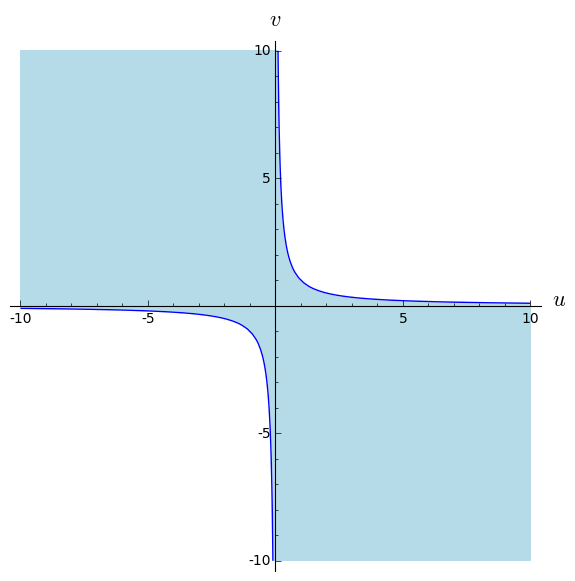
\includegraphics[width=1\textwidth]{plots/ch1_01_S_1.png}
\caption{$S_1:=\set{uv<1}$.\label{fig:S_1}}
\end{subfigure}
\begin{subfigure}{.55\linewidth}\centering
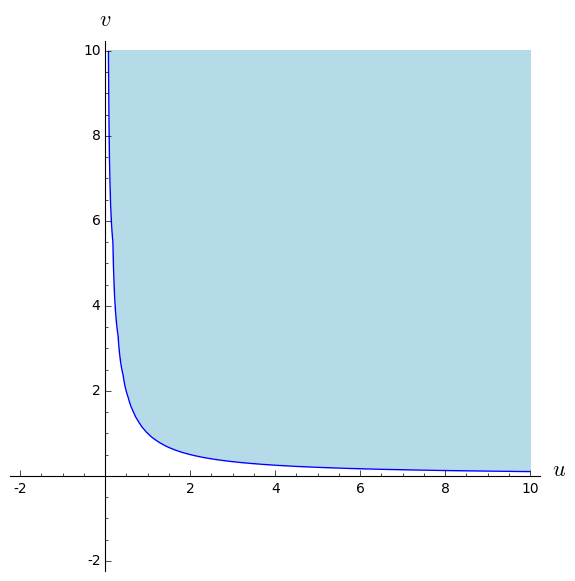
\includegraphics[width=1\textwidth]{plots/ch1_02_S_2.png}
\caption{$S_2:=\set{uv>1,u>0}$.\label{fig:S_2}}
\end{subfigure}\\[1ex]
\caption{Plots of the regions defined in Example \ref{introExample} (ii).\label{fig:introExampleii}}
\end{figure}
\item Let $S:=R^2\setminus\set{(0, 0)}$ be the punctured plane. Then $S$ is the image of the polynomial map $(x,y) \mapsto (xy-1,(xy-1)x^2-y)$.
\item Let $\H:=\set{v>0}$ be the open upper half-plane. Then $\H$ is the image of $(x,y) \mapsto (y(xy-1),(xy-1)^2+x^2)$. This implies that every open half-plane is a polynomial image of $R^2$. This is probably the simplest polynomial map whose image is $\H$.
\end{enumerate}
\end{examples}
\end{subsection}
	
\begin{subsection}{Statement of the main results}
	
The main results of this chapter are generalizations of examples (iii) and (iv) from Examples \ref{introExample}.
	
\begin{theorem}\label{finSetTh}\em Let $n\ge2$. For every finite set $F\subset R^n$, the semialgebraic set $R^n\setminus F\subset R^n$ is a polynomial image of $R^n$.\em
\end{theorem}
%\newpage
\begin{theorem}\label{openQuadGen}\em Let $n\ge 2$. For any independent linear forms $h_1,\dots,h_r$ of $R^n$, the open semialgebraic set $\set{h_1>0,\dots,h_r>0}$ is a polynomial image of $R^n$.\em
\end{theorem}
	
Before the paper \cite{fg} was published, the exterior boundary of all open sets that were known to be polynomial images of $R^2$ was Zariski-irreducible, and all of them were deformations of $\H$. J.M. Gamboa outlined the problem of finding if $\Qu=\set{x>0,y>0}$ is a polynomial image of $R^2$ or not, since its exterior boundary is Zariski-reducible. The solution of this problem is a key particular case of the content of Theorem \ref{openQuadGen}. Before that, the closest known approach to look for a solution of this problem was the transformation
$$
\psi:R^2 \to R^2,\, (x,y)\mapsto(x^4y^2,x^2y^4)
$$	
whose image is $\Qu\cup\set{(0,0)}$. The answer to the first intriguing problem in this field was given in the following theorem:
\begin{theorem}\label{openQuad}\em The first open quadrant $\Qu$ is a polynomial image of $R^2$.\em
\end{theorem}
	
\begin{remark} The first proof of Theorem \ref{openQuad} consists of two parts:
\begin{itemize}
\item Choosing a ``good'' candidate to be a polynomial map whose image is close enough to $\Qu$, and giving the reasons behind this choice (see subsection \ref{quadReasons}). 
	
\item Checking that the image of the map is $\Qu$ indeed. After some arguments, this can be reduced to prove the non-existence of real roots of certain polynomials in one variable on certain intervals, and to compare some rational functions on those intervals. In order to do this, we use symbolic computations with tools like Sage and Maple. Because of the high degree of the involved polynomials, the actual checking of the non-existence of roots is done with a Maple package that performs \hyperref[sturm]{Sturm algorithm} and a Python programme that implements Laguerre's method. %Comentar el método de Laguerre en el apéndice
\end{itemize}
\end{remark}

Let us see how Theorem \ref{openQuadGen} follows from Theorem \ref{openQuad}.
		
\vspace{1mm}		
		
[Proof of theorem \ref{openQuadGen}] After a linear change of coordinates we can suppose that $h_1:=x_1,\dots,h_r:=x_r$,  so we only have to prove that for every pair of positive integers $r\leq n$ the semialgebraic set $\{x_1>0,\dots,x_r>0\}\subset R^n$ is a polynomial image of $R^n$. This is reduced to prove the following two steps:
\begin{itemize}
\item $\H:=\{x_1>0\}$ and $\Qu:=\{x_1>0,\, x_2>0\}\subset R^2$ are polynomial images of $R^2$, which is true, respectively, by Example \ref{introExample} (iv) and Theorem \ref{openQuad}.
\item This implies that $\mathscr{O}:=\{x_1>0,\, x_2>0,\, x_3>0\}\subset R^3$ is a polynomial image of $R^3$. Indeed, let $H_1,H_2:R^2 \rightarrow R^2$ be polynomial maps whose respective images are $\H$ and $\Qu$. Let us define:
\begin{align*}
(H_1,\text{id}_R): R^3=R^2\times R\longrightarrow R^3= R^2\times R\\
(\text{id}_R,H_2): R^3=R\times R^2\longrightarrow R^3= R\times R^2.
\end{align*}
Then, $\mathscr{O}$ is the image of the polynomial map 
$$
H:=(\text{id}_R,H_2)\circ(H_1,\text{id}_R):R^3\rightarrow R^3
$$ 
\end{itemize} 
Once the case $n=3$ is solved the case of arbitrary $n$ follows straightforwardly.	\qed		

\vspace{1mm}
		
The original proofs of Theorems \ref{finSetTh} and \ref{openQuad} are written for $R:=\R$. As for both theorems explicit polynomial maps are given, the results can be extended to arbitrary real closed field $R$ by the \hyperref[TP]{Transfer Principle}.
\end{subsection}
\end{section}

\begin{section}{Complementary set of a finite set}
	
We proceed to prove theorem \ref{finSetTh}:
	
\vspace{1mm}
	
[Proof of theorem \ref{finSetTh}] Let $F:=\{p_1,\dots,p_k\}$. Let us see that it suffices to prove the result for points of the form $p_j:=(a_j,\vec{0})\in\R\times\R^{n-1}$. After a linear change of coordinates we can assume that the first coordinates of the given points are pairwise distinct. 

In other words, we denote $p_j:=(a_{1j},\dots,a_{nj})$ and we may suppose that $a_{1j}\neq a_{1\ell}$ when $j\neq\ell$. Then, there exists a polynomial $P_1\in\R[T]$ such that $P_1(a_{1j})=a_{nj}$, with $j = 1,\dots, n$, and denoting $x':=(x_1,\dots,x_{n-1})$, we  define the polynomial map 
$$
h_1:\R^n\to\R^n,\, (x',x_n)\mapsto (x',x_n+P_1(x_1)).
$$
Indeed $h_1$ is bijective. Note first that every point of $\R^n$ has a preimage in $\R^n$, namely if $x:=(x_1, \dots,x_n)$, then $z:=(x',x_n-P_1(x_1))$ satisfies $h_1(z)=x$ and $h_1$ is onto. As for being injective, let $x,y\in\R^n$ such that 
$$
h_1(x)=(x_1,\dots,x_n+ P_1(x_1))=(y_1,\dots,y_n+ P_1(y_1))=h_1(y).
$$ 
Then $x_i=y_i$ for $i=1,\dots,n-1$. Also $x_n+P_1(x_1)=y_n+P_1(y_1)$ and $P_1(x_1)=P_1(y_1)$ because $x_1= y_1$. Therefore $x_n=y_n$ and $x=y$.
		
Now, for $p_j':=(a_{1j},\dots,a_{(n-1)j},0)$ we have $h_1(p_j')=p_j$. Analogously, there exists $P_2\in\R[T]$ such that $P_2(a_{1j}) = a_{(n-1)j}$, and define the polynomial bijection
$$
h_2:\R^n\longrightarrow \R^n,\,(x'',x_{n-1},x_n)\mapsto (x'',x_{n-1}+P_2(x_1),x_n),
$$
where $x''=(x_1,\dots,x_{n-2})$. Then $h_2(p_j'')=p_j'$ for $p_j''= (a_{1j},\dots,a_{(n-2)j},0,0)$. In this way the polynomial bijection $h_1\circ h_2:\R^n\to\R^n$ satisfies
$$
(h_1\circ h_2)(p_j'')=h_1(h_2(p_j''))=h_1(p_j')=p_j,
$$
and we can inductively construct a polynomial bijection $h:\R^n\rightarrow\R^n$ such that $h(q_j)=p_j$ for $q_j:=(a_{1j},\vec{0})\in\R\times\R^{n-1}$. Now let $G:=\{q_1,\dots,q_k\}$ and suppose that there exists a polynomial map $g:\R^n\rightarrow\R^n$ such that $g(\R^n)=\R^n\setminus G$. Then $(h\circ g)(\R^n) = \R^n \setminus F$, which concludes the first part of the proof. Thus in what follows we suppose that $p_j=(a_j,\vec{0})$.
		
We claim that the image of the polynomial map $f:=(f_1,\dots,f_n)$:
$$
f(x)=\left(x_1x_2-r+a_1,\ x_1^{4}\rho(x)+x_1^{2}\sigma(x)+x_2,\ x_3,\dots,\ x_n\right)
$$
is $\R^n\setminus F$, where $r$ is an integer such that $r\neq a_1-a_j$ for $j=1,\dots,k$,  
$$
\sigma(x):=\sum_{j=3}^n x_j^2 \text{ and } \rho(x):=\prod_{j=1}^k(x_1x_2-r+a_1-a_j).
$$
First, suppose that there exists $b:=(b_{1},\dots,b_{n})\in R^n$ such that $f(b)=p_\ell$ for some $\ell=1,\dots,k$. Then $f_1(b)=b_1b_2-r+a_1=a_\ell$. Thus the $\ell^{th}$-factor of the polynomial $\rho$ evaluated at $x:=b$ is
$$
b_1b_2-r+a_1-a_\ell=a_\ell-a_\ell=0,
$$		 
and $\rho(b)=0$. In addition, the equality $f(b)=p_\ell=(a_{_\ell},\vec{0})$ implies that $f_i(b)=0$ for $i=2,\dots,n$. In particular, since $f_i\equiv\text{id}$ for $i=3,\dots,n$ we get $b_i=0$ for $i=3,\dots,n$. Hence $\sigma(b)=0$. As $\sigma(b)=\rho(b)=0$ we get $b_2=f_2(b)= 0$, so $b_2=0$ and $a_{\ell}=f_1(b)=a_1-r$, that is, $r=a_1-a_\ell$, which is a contradiction. So $\text{im}(f)\subset \R^n\setminus F$.
Conversely, let $u:=(u_1,\dots,u_n)\in\R^n\setminus F$. We must prove that the system of polynomial equations:
\[ \left\{ \def\arraystretch{1.2}
\begin{array}{ll} 
f_1(x)&=x_1x_2-r+a_1=u_1 \\
f_2(x)&=x_1^4\rho(x)+x_1^2\sigma(x)+x_2=u_2 \\
f_j(x)&=x_j=u_j,\quad j\geq 3
\end{array} 
\right.  \]
has a solution.
\begin{enumerate}[(i)]
\item If $u_1=a_1-r$ then $f(0,u_2,\dots,u_n)=u$.
\item If $u_1\neq a_1-r$ we use the first equation to substitute $$x_2=\frac{u_1-a_1+r}{x_1} \quad \text{ and } \quad x_j=u_j \quad \text{ for } j\geq 3.$$ Now, we expand $f_2(x)$:
$$
x_1^4\rho(x)+x_1^2\sigma(x)-u_2=-x_2=-\frac{u_1-a_1+r}{x_1}
$$ 
and multiplying by $x_1$ we get 
$$
x_1^5\rho(x)+x_1^3\sigma(x)-u_2x_1+(u_1-a_1+r)=0.
$$ 
Then, $\rho(x)=\prod_{j=1}^k(u_1-a_j) \text{ and } \sigma(x)=\sigma(u)$. Now it is clear that $x_1$ must be a nonzero root of the polynomial:
$$
Q(T)=\Big(\prod_{j=1}^k(u_1-a_j)\Big)T^{5}+\sigma(u)T^{3}-u_2T+(r-a_1+u_1),
$$
which has odd degree, and so a real root, unless 
$$
\prod_{j=1}^k(u_1-a_j)=\sigma(u)=u_2=0.
$$ 
If this were the case, then $u_1=a_j$ for some $j= 1,\dots,k$ and $u_2=u_3=\cdots=u_k=0$. This is not possible because $u\not\in F$. Thus, $Q(T)$ has a real root $b_1$, and in fact $b_1\neq0$ because $Q(0)=r-a_1+u_1\neq 0$.
Finally, 
$$
f\left(b_1,\ \frac{u_1-a_1+r}{b_1},\ u_3,\ \dots,\ u_n\right)=u,
$$
as required.
\end{enumerate}
\qed
\end{section}

\begin{section}{The open quadrant $\Qu$ problem}
\begin{subsection}{Reasons behind the choice}\label{quadReasons}
		
It is remarkable that even though the open interval $I:=(0,+\infty)$ is the image of $\R^2$ under the polynomial map $h:\R^2\to\R,\, (x,y)\mapsto (xy-1)^2+x^2$, see fig. \ref{fig:h(x,y)}, the interval $I$ is not a polynomial image of $\R$ because polynomial images of the real line are closed subsets of $\R$.
\begin{figure}[h]
\begin{center}
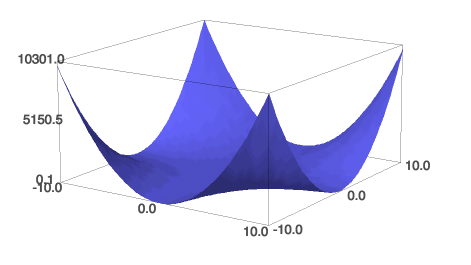
\includegraphics[width=0.8\textwidth]{plots/ch1_03_f(x,y).png}
\caption{$h(x,y)=(xy-1)^2+x^2$.\label{fig:h(x,y)}}
\end{center}
\end{figure}
		
However, although $h(\R^2)=I$, the polynomial $h$ does not help to obtain $\Qu$ at all:
\begin{remark}
There is no polynomial map $f:=(P_1, P_2):\R^2\to\R^2$ satisfying $f(\R^2)=\Qu$ and $P_1(x,y)=(xy-1)^2+x^2$.
\end{remark}
The proof of this remark relies on a suitable use of the Curve Selection Lemma (\cite[VIII.2.6]{abr}) to approach a point $(\lambda^2,0)\in\overline{\Qu}$ with $\lambda>0$, to get a contradiction.
		
On the topic of finding a polynomial map $\Phi:\R^2\to\R^2$ that satisfies $\Phi(\R^2)=\Qu$, ``a major difficulty" is the following:
\begin{center}
\begin{tabular}{rr}
$\qquad \qquad\quad$ \fbox{\textit{The closure of its image must contain the positive half-axes.}} & $\quad \quad$ ($\clubsuit$)
\end{tabular}
\end{center}
\begin{remark} Using Theorem \ref{finSetTh}, we just need to find a polynomial map $$\P=(\F,\G):\R^2\to\R^2$$ such that $\P(\R^2)$ is the disjoint union of $\Qu$ and a set with finite preimage, say $\P(\R^2)=\Qu\ \sqcup F$ with $\P^{-1}(F)$ a finite set. By Theorem \ref{finSetTh} there exists a polynomial map $\varphi:\R^2\to\R^2$ such that $\varphi(\R^2)=\R^2\setminus\P^{-1}(F)$ and the polynomial map $\Phi:=\P\circ\varphi$ satisfies
$$
\Phi(\R^2)=\P(\varphi(\R^2))=\P(\R^2\setminus\P^{-1}(F))=\P(\R^2)\setminus F=(\Qu\ \sqcup F)\setminus F=\Qu.
$$ 
\end{remark}
We are going to define a map $\P:=(\F,\G)$ that accomplish this task, with $F:=\set{(-1,0),(0,-1)}$. If we were able to find such map $\P$, then condition ($\clubsuit$) will immediately be satisfied. 
		
Suppose for a while that such a map $\P$ exists. Then, for every $\lambda,\mu\ge 0$ there will exist \hyperref[curveGerms]{Nash half-branch curve germs} $\alpha_{\lambda}(s),\beta_{\mu}(s)$ which cannot be extended to $0$ and such that:
$$
\lim_{s\rightarrow 0} P(\alpha_{\lambda}(s))=(\lambda^2,0)\qquad \text{and} \qquad \lim_{s\rightarrow 0} P(\beta_{\mu}(s))=(0,\mu^2).
$$
We can try parameterizations of the form:
$$
\alpha_{\lambda}(s):=\left(s^{n_{\lambda}},\frac{a_{\lambda 0}+a_{\lambda 1}s+\cdots}{s^{m_{\lambda}}}\right)
\quad \text{ and } \quad
\beta_{\mu}(s):=\left(\frac{b_{\mu 0}+b_{\mu 1}s+\cdots}{s^{\ell_{\mu}}},s^{k_{\mu}}\right).
$$
Then $a_{\lambda 0},b_{\mu 0}$ must be constants (except maybe for finitely many values of $\lambda$ and $\mu$). This leads us to choose curves of the type:
$$
\alpha_{\lambda}(s):=\left(s^{n_{\lambda}},\frac{1+a_{\lambda 1}s+\cdots}{s^{m_{\lambda}}}\right)
\quad \text{ and } \quad
\beta_{\mu}(s):=\left(\frac{1+b_{\mu 1}s+\cdots}{s^{\ell_{\mu}}},s^{k_{\mu}}\right),
$$
and among them we make the simplest choice: 
$$
\alpha_{\lambda}(s):=\left(s,\frac{1+a_{\lambda }s}{s}\right)
\quad \text{ and } \quad
\beta_{\mu}(s):=\left(\frac{1+b_{\mu }s}{s},s^{3}\right).
$$
The following pair of polynomials:
\begin{equation*}
\boxed{
\begin{aligned}
\F(x,y)&:=(1-x^3y+y-x y^2)^2+(x^2 y)^2&=&\ \F_1^2+\F_2^2 \\
\G(x,y)&:=(1-xy+x-x^4y)^2+(x^2y)^2&=&\ \G_1^2+\G_2^2\\
\end{aligned}
}
\end{equation*}
enjoy a nice behavior along these curves, as the following images show:

\begin{figure}[h]\hspace{-0.5cm}
\begin{subfigure}{.54\linewidth}\centering
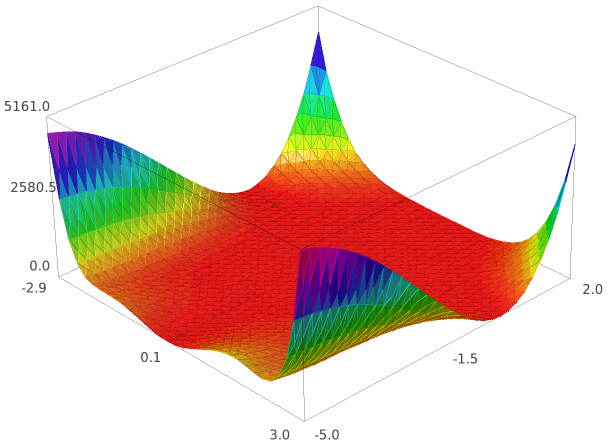
\includegraphics[width=1\textwidth]{plots/ch1_04_F.png}
\caption{$\F(x,y):=(1-x^3y+y-xy^2)^2+(x^2y)^2$.\label{fig:F}}
\end{subfigure}
\begin{subfigure}{.55\linewidth}\centering
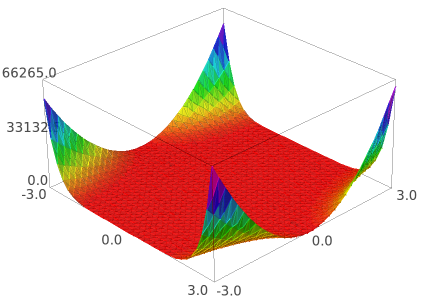
\includegraphics[width=1\textwidth]{plots/ch1_05_G.png}
\caption{$\G(x,y)=(1-xy+x-x^4y)^2+(x^2y)^2$.\label{fig:G}}
\end{subfigure}\\[1ex]
\caption{Plots of the polynomials $\F,\G:\R^2\longrightarrow\R$.\label{fig:plotFG}}
\end{figure}
Next, notice that
\begin{enumerate}[(a)]
\item $\cdot$ $\F_1\circ\alpha_\lambda=1-a_{\lambda}-a_{\lambda}^{2} s-s^{2}-a_{\lambda} s^{3}\in\R[s,a_{\lambda}]$,
$\, \F_1\circ\alpha_{\lambda }(0)=1-a_{\lambda. }$ \newline
$\cdot$ $\F_1\circ\beta_{\mu}=-3\,b_{\mu}s-3 \,b_{\mu}^{2} s^{2}-{\left(b_{\mu}^{3}-1\right)}s^{3}-s^{5}-b_{\mu}s^{6}\in\R[s,b_{\mu}]$,
$\, \F_1\circ\beta_{\mu}(0)=0$.
				
\item $\cdot$ $ \G_1\circ\alpha_{\lambda } = {\left(1-a_{\lambda} \right)}s-s^{3}-a_{\lambda} s^{4} \in\R[s,a_{\lambda}]$,
$\, \G_1\circ\alpha_{\lambda }(0)=0$.

$\cdot$ $\G_1\circ\beta_{\mu}=1-3\, b_{\mu}-6\,b_{\mu}^{2}s-{\left(4\,b_{\mu}^{3}+1\right)}s^{2}-{\left(b_{\mu}^{4}+ b_{\mu}\right)}s^{3}\in\R[s,b_{\mu}]$, \text{ and } $\ \ \G_1\circ\beta_{\mu}(0)=1-3b_{\mu}$.
		
\item $\cdot$ $\F_2\circ\alpha_{\lambda }= s+a_{\lambda} s^{2} = \G_2\circ\alpha_{\lambda}\in\R[s,a_{\lambda }]$.
			
$\cdot$ $\F_2\circ\beta_{\mu}= s+2 \, b_{\mu} s^{2}+b_{\mu}^{2} s^{3} = \G_2\circ\beta_{\mu}\in\R[s,b_{\mu}]$.
				
$\cdot$ $\F_2\circ\alpha_{\lambda }(0)=\G_2\circ\alpha_{\lambda}(0)=\F_2\circ\beta_{\mu}(0)=\G_2\circ\beta_{\mu}(0)=0$.
\end{enumerate}
All of these map compositions were computed by Sage. Thus, we get the following properties:
		
\begin{enumerate}[(i)]
		
\item The polynomials $\F,\G$ are non-negative in $\R^2$.
		
\item $\cdot$ $\F^{-1}(0)=\F_1^{-1}(0)\cap \F_2^{-1}(0)=\{(0,-1)\}\xmapsto{\ \P\ }\set{(0,1)}$.
			
$\cdot$ $\G^{-1}(0)=\G_1^{-1}(0)\cap \G_2^{-1}(0)\ =\, \{(-1,0)\} \xmapsto{\ \P\ } \set{(1,0)}$.
		
\item $\cdot$ $\P\circ\alpha_{\lambda}=(\F\circ\alpha_{\lambda },\G\circ\alpha_{\lambda})=$
			
$\arraycolsep=2pt\def\arraystretch{1.2}
\begin{array}{l}
\left(\right.a_{\lambda}^{2}-2 \,a_{\lambda}+1+2 \,{(a_{\lambda}^{3}-a_{\lambda}^{2})}s+{(a_{\lambda}^{4}+2 \, a_{\lambda}-1)} s^{2}+ \,a_{\lambda}^{2} s^{3}+\\
\quad {(2\, a_{\lambda}^{3}+a_{\lambda}^{2}+1)}s^{4}+2 \,a_{\lambda} s^{5}+a_{\lambda}^{2} s^{6},\\		
\ {(a_{\lambda}^{2}-2 \ a_{\lambda}+2)} s^{2}+2 \, a_{\lambda} s^{3}+{(a_{\lambda}^{2}+2 \,a_{\lambda}-2)}s^{4}+\\
\quad \,2 \,{(a_{\lambda}^{2}-a_{\lambda})}s^{5}+s^{6}+2\,a_{\lambda} s^{7}+a_{\lambda}^{2}s^{8}\left.\right).
\end{array}
$
				
$\cdot$ $\P\circ\beta_{\mu}=(\F\circ\beta_{\mu},\G\circ\beta_{\mu})=
$
				
				$\arraycolsep=2pt\def\arraystretch{1.2}
\begin{array}{l}
\left(\right.{(9 \,b_{\mu}^{2}+1)}s^{2}+2 \,{(9 \,b_{\mu}^{3}+2\,b_{\mu})}s^{3}+3\,{(5\,b_{\mu}^{4}+2\,b_{\mu}^{2}-2\,b_{\mu})}s^{4}+\\
\quad 2\,{(3 \,b_{\mu}^{5}+2\,b_{\mu}^{3}-3\,b_{\mu}^{2})}s^{5}+{(b_{\mu}^{6}+b_{\mu}^{4}-2\,b_{\mu}^{3}+6\,b_{\mu}+1)} s^{6}+\\
\quad 12\,b_{\mu}^{2} s^{7}+2\,{(4\,b_{\mu}^{3}-1)}s^{8}+2\,{(b_{\mu}^{4}-b_{\mu})}s^{9}+s^{10}+2\,b_{\mu}s^{11}+b_{\mu}^{2} s^{12},\\
					\ 9 \, b_{\mu}^{2}-6 \, b_{\mu}+1+12 \, {(3 \, b_{\mu}^{3} - b_{\mu}^{2})} s+{(60\, b_{\mu}^{4} - 8 \, b_{\mu}^{3}+6 \, b_{\mu}-1)}s^{2} + \\
					\quad 2 \, {(27\,b_{\mu}^{5}-b_{\mu}^{4}+9\,b_{\mu}^{2}+b_{\mu})}s^{3}+{(28\,b_{\mu}^{6}+20\,b_{\mu}^{3}+6\,b_{\mu}^{2}+1)} s^{4}+\\
					\quad2\,{(4\,b_{\mu}^{7}+5\,b_{\mu}^{4}+2\,b_{\mu}^{3}+b_{\mu})}s^{5}+{(b_{\mu}^{8}+2\,b_{\mu}^{5}+ b_{\mu}^{4} +b_{\mu}^{2})} s^{6}\left.\right).
					\end{array}
$
\end{enumerate}
The polynomials $\F\circ\alpha_{\lambda },\ \G\circ\alpha_{\lambda}\in\R[s,a_{\lambda}]$ and $\F\circ\beta_{\mu},\ \G\circ\beta_{\mu}\in\R[s,b_{\mu}]$ were computed with Sage. As we anticipated before, by condition (ii) the set $F=\set{(-1, 0),(0,-1)}$.
\end{subsection}
\begin{subsection}{The proof} [Proof of theorem \ref{openQuad}] We are going to prove that $\Qu\subset\P(\R^2)$. To do this it is enough to fix $v>0$ and see that the image under $\F$ of the curve $\{\G=v\}$ contains the open half-line $(0,+\infty)$.
\begin{center}
\fbox{\textbf{Step 1}} \emph{Parametrization of the curve $\{\G-v=0\}$.}
\end{center}\label{step1}

We start by solving the equation $\G-v=0$, that is, 
$$
(1-xy+x-x^4y)^2+(x^2y)^2-v=0
$$ 
As it has degree $2$ with respect to $y$, we can compute its roots $y^+(x,v)$ and $y^-(x,v)$ given by:
\begin{equation*}
\begin{aligned}
y^+(x,v)&:=\frac{1+x+x^3+x^4+\sqrt{\Delta(x,v)}}{x(x^2+(x^3+1)^2)}\\
y^-(x,v)&:=\frac{1+x+x^3+x^4-\sqrt{\Delta(x,v)}}{x(x^2+(x^3+1)^2)}\\
\end{aligned}
\end{equation*}
where $\Delta(x,v)=\Delta_v(x):=v(x^2+(x^3+1)^2)-x^2(x+1)^2,\ \text{deg}_x(\Delta)=6$. We can see on figure \ref{fig:plotYs_1} how $y^+$ and $y^-$ look like for instance for $v:=0.8$. As we can see on figure \ref{fig:plotYs_2}, for $v:=1$ there are no singularities on $y^-$ because $\lim_{x\rightarrow0}y^-(x,1)=1$. This observation is used later, in \hyperref[step2]{Step 2}.
\begin{figure}[h]
\centering
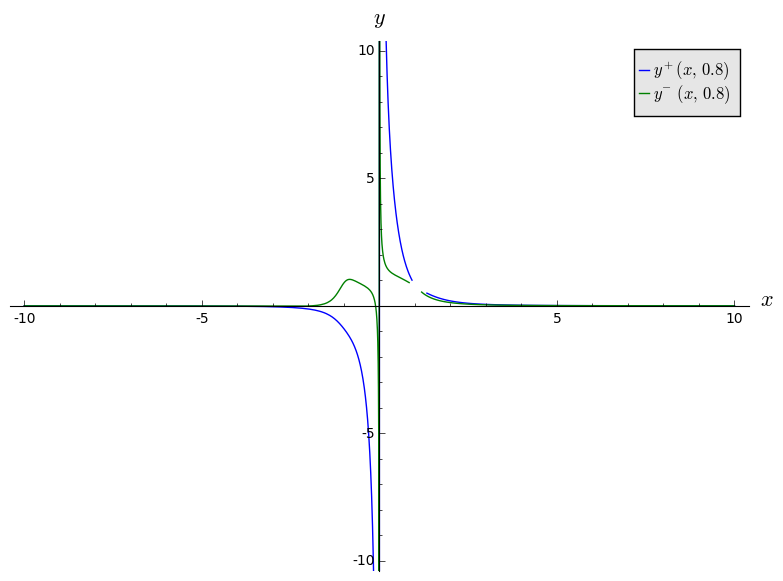
\includegraphics[width=1\textwidth]{plots/ch1_06_sols.png}
\caption{$y^+(x,v)$ and $y^-(x,v)$ for $v:= 0.8$.\label{fig:plotYs_1}}
\end{figure}
\begin{figure}[h]
\centering
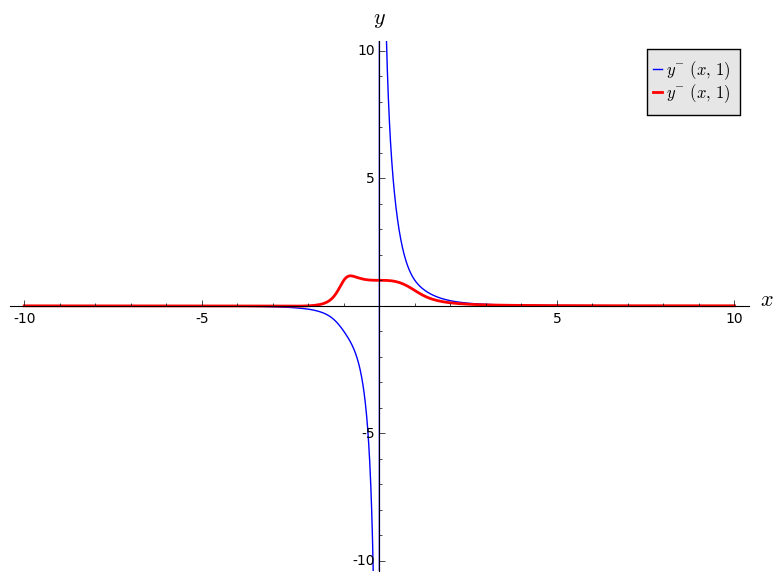
\includegraphics[width=1\textwidth]{plots/ch1_07_sols_1.png}
\caption{$y^+(x,v)$ and $y^-(x,v)$ for $v:=1$.\label{fig:plotYs_2}}
\end{figure}

The common domain of these two functions is the set 
$$
D_v:=\{x\in R:\, \Delta(x,v)\geq 0,\,x\neq 0\}.
$$ 
Notice that the only real root of the denominator is $x_0:=0$\footnote{We checked with Laguerre's method, implemented with Python 2.7, that the polynomial $x^7+2x^4+x^3+x$ has 6 complex roots.} Let
$$
\gamma_v^+: D_v\to\R,\, x\mapsto\F(x,y^+(x,v))\quad\text{ and }\quad\gamma_v^-:D_v\to\R,\, x\mapsto\F(x,y^-(x,v))
$$
Notice that $\F(\set{\G=v})=\text{im}(\gamma_v^+)\cup\text{im}(\gamma_v^-)$, so our aim is to prove that $(0,+\infty)\subset\text{im}(\gamma_v^+)\cup\text{im}(\gamma_v^-)$.
\begin{center}
\fbox{\textbf{Step 2}} \emph{Main properties of $\gamma_v^+ \text{ and } \gamma_v^-$.}
\end{center}\label{step2}
In this section we are going to prove that:
$$
\text{(i)} \lim_{x\rightarrow \pm\infty}\gamma_v^+(x)=\lim_{x\rightarrow \pm\infty}\gamma_v^-(x)=0.
$$
$$\text{(ii)} \lim_{x\rightarrow 0}\gamma_v^+(x)=+\infty
,\quad \lim_{x\rightarrow 0}\gamma_v^-(x)=\left\{\begin{array}{ll}
+\infty&\text{ for $v\neq 1$}\\
 4 & \text{ for $v=1$}
\end{array} \right.
$$
Using Sage we can symbolically check how $\gamma_v^+\text{ and }\gamma_v^-$ look like, getting polynomials $A_1,A_2,B_1,B_2\in\R[x,v]$ and $C\in \R[x]$ such that:
$$\text{(a) }\gamma_v^+(x)=\dfrac{A_1(x,v)+B_1(x,v)\sqrt{\Delta(x,v)}}{C(x)}, \ \ 
\gamma_v^-(x)=\dfrac{A_2(x,v)+B_2(x,v)\sqrt{\Delta(x,v)}}{C(x)}$$
$$
\text{(b)}\ \ 
\arraycolsep=1.4pt\def\arraystretch{1.5}
\begin{array}{cclrl}
A_1(x,v)&=&\ \ A_2(x,v)\, , & \text{deg}_x(A_1)=\text{deg}_x(A_2)=24& \\
B_1(x,v)&=&-B_2(x,v)\, , &\text{deg}_x(B_1)=\text{deg}_x(B_2)=21& \\
C(x)&=&x^2(x^2+(x^3+1)^2)^4\, , & \text{deg}_x(C)=26&.
\end{array}
$$
We proceed to study $\gamma_v^+$ and $\gamma_v^-$ at the origin. Since $\Delta$ has even degree and positive leading coefficient with respect to $x$, it is positive for $\abs{x}$ large enough, so (i) holds.
			
Now, for $x=0$, we get $\Delta(0,v)=v>0$, so $0\in\overline{D_v}$. Also:
\begin{itemize}
\item $A_1(0,v)+B_1(0,v) \sqrt{\Delta(0,v)}= v(1+\sqrt{v})^2>0$.
				\item $A_2(0,v)+B_2(0,v)\sqrt{\Delta(0,v)}=v(1-\sqrt{v})^2\geq 0$, and equality holds if and only if $v=1$.
\end{itemize}
			
\begin{figure}[h]
\centering
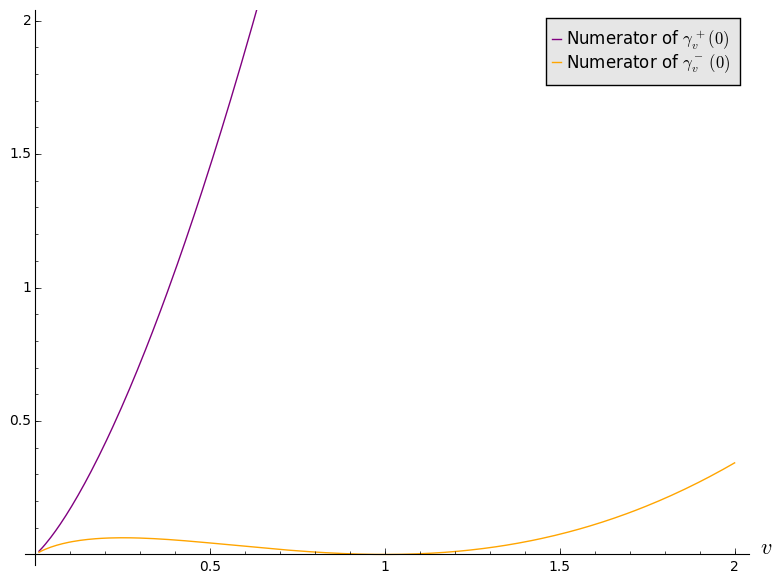
\includegraphics[width=0.75\textwidth]{plots/ch1_08_numerators.png}
\caption{Numerators of $\gamma_v^+$ and $\gamma_v^-$ for $x:=0$.\label{fig:numerators}}
\end{figure}
			
Thus, (ii) holds (we also checked it with Sage). The result for $v:=1$ in (ii) is not relevant here (see figure \ref{fig:limit}).
\begin{figure}[h]
\centering
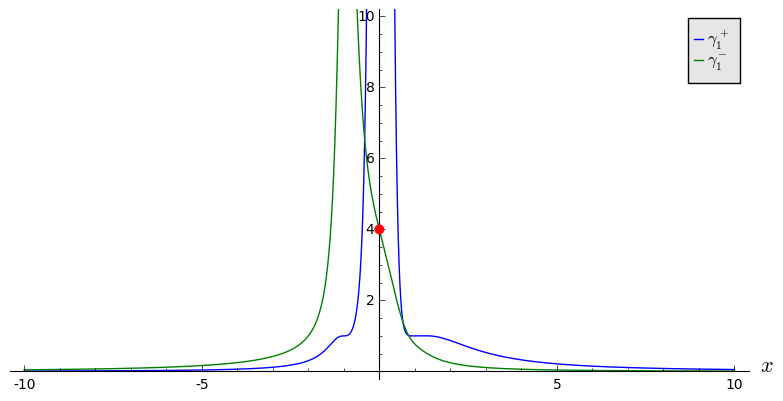
\includegraphics[width=1\textwidth]{plots/ch1_09_limit.png}
\caption{Notice the value of $\gamma_1^-(x)$ at $x=0$.\label{fig:limit}}
\end{figure}

\begin{center}
\fbox{\textbf{Step 3}} \emph{When $v\geq 0.28^2$ we have} $(0,+\infty)\subset\text{im}(\gamma_v^+)$.
\end{center}\label{step3}
In order to see whether $(0,+\infty)\subset\text{im}(\gamma_v^+)\cup\text{im}(\gamma_v^-)$ or not we are now going to study the domain $D_v$. To that end we need to study when $\Delta(x,v)=0$, so it seems convenient to define:
$$
v(x):=\frac{x^2(x+1)^2}{x^2+(x^3+1)^2},
$$
whose graph can be seen in figure \ref{fig:v(x)}. If $x\in(-\infty,0)$ we checked using Laguerre's method that the polynomial
\begin{figure}[h]\hspace{-1.75cm}
\begin{subfigure}{.6\linewidth}\centering
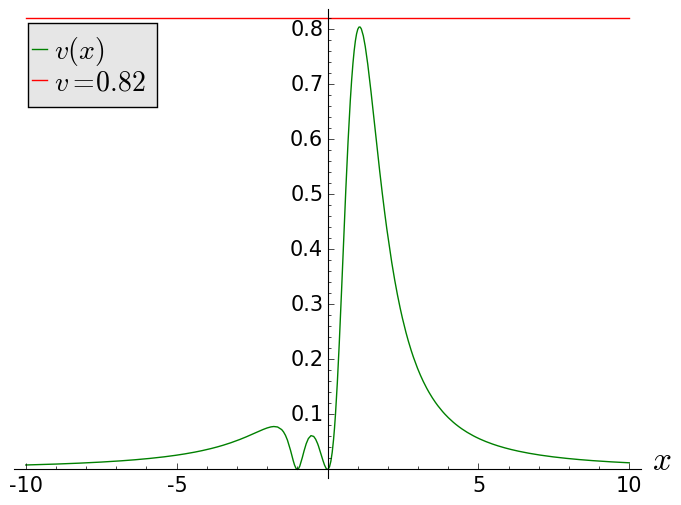
\includegraphics[width=1\textwidth]{plots/ch1_10_uve.png}
\caption{Plot of $v(x)$.\label{fig:uve}}
\end{subfigure}
\begin{subfigure}{.6\linewidth}\centering
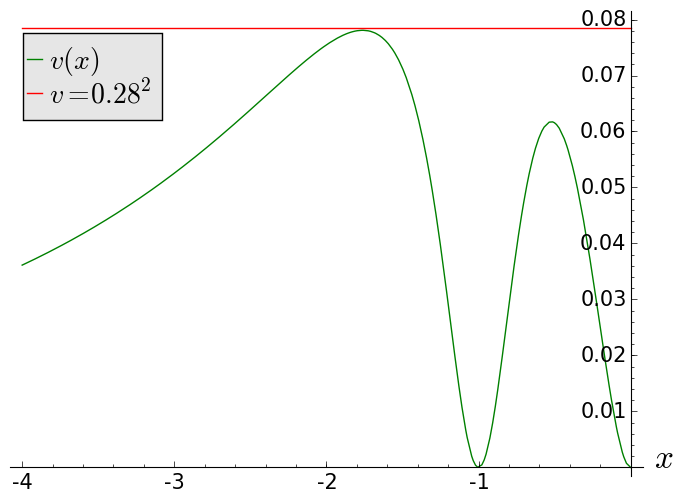
\includegraphics[width=1\textwidth]{plots/ch1_11_uve_detail.png}
\caption{Detail of the function when $x\in(-4,0)$.\label{fig:uveDetail}}
\end{subfigure}\\[1ex]
\caption{Plot of the univariate function $v(x)$.\label{fig:v(x)}}
\end{figure}
$$
\Delta(x,0.28^2)=0.0784\,x^{6}-x^{4}-1.8432\,x^{3}-0.9216\,x^{2}+0.0784
$$ 
has 4 complex roots and 2 real ones\footnote{The value $v_0:=0.28^2$ comes from a careful observation of the plot from figure \ref{fig:uveDetail}.}, with the real ones being $\delta_0\approx 0.236$ and $\delta_1\approx 4.336$. Thus $\Delta(x,v)$ has no negative roots when $v\ge 0.28^2$ and, in addition, it is positive. Therefore $(-\infty,0)\subset D_v$. But then, as $\gamma_v^+$ is continuous and recalling the limits computed in \hyperref[step2]{Step 2}, we get  
$$
(0,+\infty)\subset\text{im}(\gamma_v^+)\subset\text{im}(\gamma_v^+)\cup\text{im}(\gamma_v^-).
$$
\begin{center}
\fbox{\textbf{Step 4}} \emph{When $0<v<0.28^2$ we have} $(0,+\infty)\subset\text{im}(\gamma_v^-)$.
\end{center}
\label{step4}
To prove that for $0<v<0.28^2$ the inclusion $(0,+\infty)\subset\text{im}(\gamma_v^-)$ holds it is enough to prove the existence of $N_v,\delta_v\in\R$ satisfying			
\begin{equation*}\qquad \quad
\qquad\quad\boxed{N_v<\delta_v,\ \ (-\infty,N_v]\cup[\delta_v,+\infty)\subset D_v\text{ and } \gamma_v^-(N_v)>\gamma_v^+(\delta_v)\\
}\qquad \qquad (\spadesuit)
\end{equation*}
\begin{figure}[h]
\centering
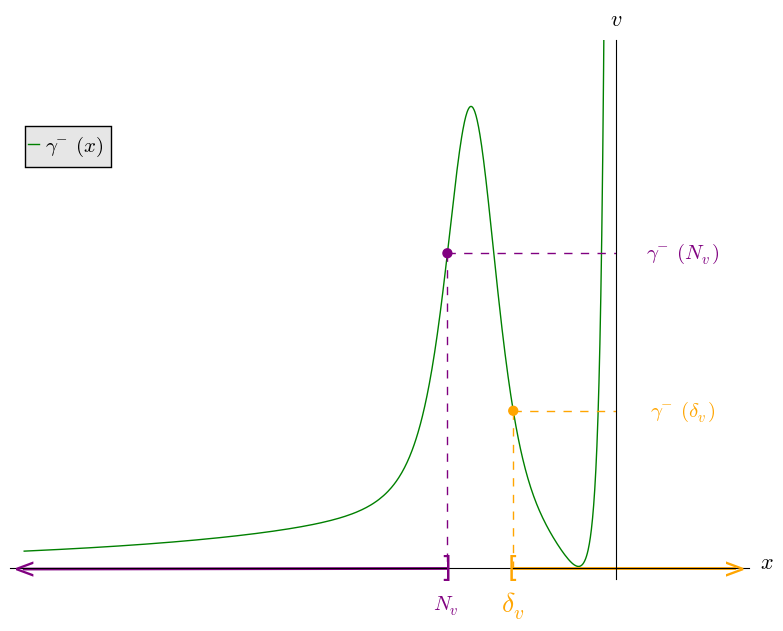
\includegraphics[width=1\textwidth]{plots/ch1_12_idea.png}
\caption{Idea of what we are saying with $(\spadesuit)$. Here $v:=0.1$.\label{fig:idea}}
\end{figure}
See figure \ref{fig:idea} to get an idea of what we are saying here. 

To prove the existence of such $N_v$ and $\delta_v$, we must compute the roots of $\Delta_v(x)$ in an algebraic closure of the field of rational functions $\R(v)$. Such an algebraic closure is the field of Puiseux series $\C\left(\set{v^*}\right)$, see \ref{puiseux}. These roots are power series in $\C\left(\set{w^*}\right)$ with $w:=\sqrt{v}$, and we consider the largest and the smallest negative roots $\eta_v,\xi_v\in\R\left(\set{v^*}\right)$ of $\Delta_v$ with respect to the unique ordering in $\R\left(\set{v^*}\right)$ that makes $v$ positive and infinitesimal with respect to $\R$. These roots are:
			
\begin{equation*}\left\{\begin{split}
\eta_v:=&-\frac{1}{w}+1+w+w^2+\frac{5}{2}w^3+\cdots\\
\xi_v:=&-w-w^2-\frac{5}{2}w^3-6w^4+\cdots
\end{split}\right.
\end{equation*}
Notice that, by the definition of the ordering in $\R\left(\set{v^*}\right)$, the first coefficient of a series is the ``most meaningful orderwise". In particular $\eta_v<\xi_v$. To perform calculations, we handle suitable truncations of the involved series. Here the word suitable means ``as short as possible but order preserving"; in other words, we look for $N_v$ and $\delta_v$ with $N_v<\eta_v<\xi_v<\delta_v$, and in fact we choose
\begin{equation*}\left\{
\begin{split}
N_v:=&-\frac{1}{w}+1+w+w^2=\eta_v-\Big(\frac{5}{2}w^3+\cdots\Big)<\eta_v\\
\delta_v:=&-w-w^2-\frac{5}{2}w^3=\xi_v-(-6w^4+\cdots)>\xi_v
\end{split}\right.
\end{equation*}
We checked with Sage that $-\infty<N_v<\delta_v<0$ for $v\in (0,0.28^2)$ that is, for $w\in(0,0.28)$, see fig. \ref{fig:comp}. Now we can focus on proving $(\spadesuit)$. Since $\Delta(N_{w^2},w^2)$ and $\Delta(\delta_{w^2},w^2)$ are positive (see fig. \ref{fig:positive}) for $w\in (0,0.28)$, we get that $N_v, \delta_v\in D_v$.
\begin{figure}[h]\hspace{-1.25cm}
\begin{subfigure}{.56\linewidth}\centering
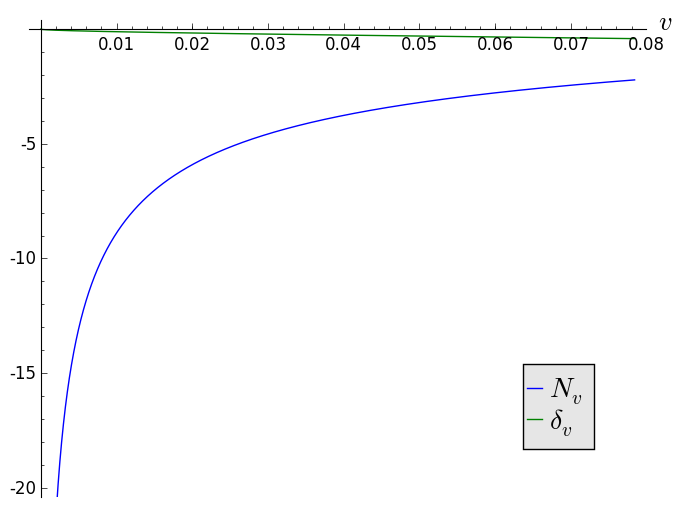
\includegraphics[width=1\textwidth]{plots/ch1_13_comp.png}
\caption{$-\infty<N_v<\delta_v<0$.\label{fig:comp}}
\end{subfigure}
\begin{subfigure}{.6\linewidth}\centering
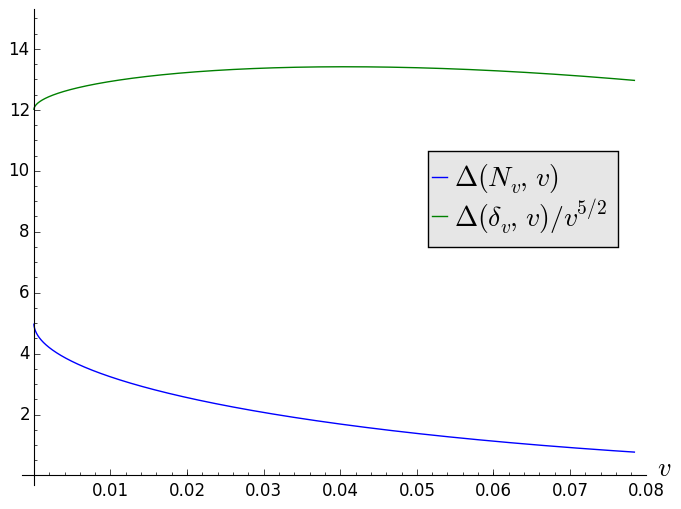
\includegraphics[width=1\textwidth]{plots/ch1_14_positive.png}
\caption{$\Delta(N_{v}, v), \Delta(\delta_{v},v) > 0$.\label{fig:positive}}
\end{subfigure}\\[1ex]
\caption{Plots of $N_v,\delta_v<0$ and $\Delta(N_{v},v),\ \Delta(\delta_{v},v)>0$ for $v\in(0, 0.28^2)$.\label{fig:N_delta}}
\end{figure} For the first part, let 
$$
D:=\bigcup_{v>0}D_v=\bigcup_{v>0}\set{x\in\R:\Delta(x,v)\geq 0,\,x\neq 0},
$$ 
whose boundary is the union of the axis $\{x=0\}$ and the curve given by the equation $\Delta(x,v)=0$, that is, the graph of the regular function
$$
v(x)=\frac{x^2(x+1)^2}{x^2+(x^3+1)^2}.
$$
This graph is above the axis $\{v=0\}$. Then, $(-\infty,N_v]$ and $[\delta_v,0)$ are contained in the interior of $D_v$ for $v\in (0, 0.28^2)$, because the curves 
$$
\set{(\delta_v,v):0<v<0.28^2} \quad\text{ and }\quad \set{(N_v,v):0<v<0.28^2}
$$ 
are contained in $D$, they are graphs above the vertical axis $\{x=0\}$, and $\delta_v<\xi_v$ and $N_v<\eta_v$ as we saw before. Look at figure \ref{fig:nice_plot}.

\begin{figure}[h]
\centering
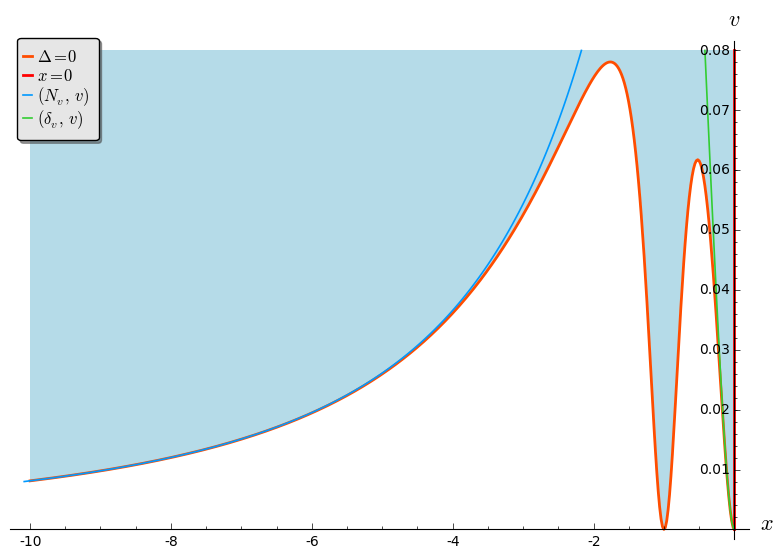
\includegraphics[width=1\textwidth]{plots/ch1_15_nice_plot.png}
\caption{Plot of $\set{(N_v, v)}, \set{(\delta_v,v)}\subset D_v$, for $0<v<0.28^2$.\label{fig:nice_plot}}
\end{figure}
So the only thing left to do is checking that $\gamma_v^-(N_v)>\gamma_v^-(\delta_v)$. Recall that 
$$
\gamma_v^-(x)=\dfrac{A_2(x,v)+B_2(x,v)\sqrt{\Delta(x,v)}}{C(x)},
$$
with $\text{deg}_x(A_2)=24,\text{deg}_x(B_2)=21, \text{deg}_x(\Delta)=6 \text{ and }\text{deg}_x(C)=26$. Consider:
$$
\arraycolsep=2pt\def\arraystretch{1.5}
\begin{array}{rclcrcl}
\cdot\ f_1(w)&=&A_2(N_{w^2},w^2)\cdot w^{24}& \qquad &\cdot\ f_2(w)&=& A_2(\delta_{w^2},w^2)\\
\cdot\ g_1(w)&=&B_2(N_{w^2},w^2)\cdot w^{21}& \qquad &\cdot\ g_2(w)&=&B_2(\delta_{w^2},w^2)\\
\cdot\ q_1(w)&=&\Delta(N_{w^2},w^2)& \qquad &\cdot\ q_2(w)&=&\Delta(\delta_{w^2},w^2)\\
\cdot\ h_1(w)&=&C(N_{w^2})\cdot w^{26}& \qquad &\cdot\ h_2(w)&=&C(\delta_{w^2}).
\end{array}
$$
Thus, we need to prove that for $w\in(0,0.28)$:
$$
\frac{f_1\cdot(w^{24})^{-1}+g_1\cdot (w^{21})^{-1}\sqrt{q_1}}{h_1\cdot(w^{26})^{-1}}>\frac{f_2+g_2\sqrt{q_2}}{h_2} \iff
$$
$$
\frac{w^2h_2f_1-f_2h_1}{h_1h_2}+\frac{w^5g_1\sqrt{q_1}}{h_1}-\frac{g_2\sqrt{q_2}}{h_2}>0,
$$
and we are going to prove that 
$$
\Lambda_1:= \frac{w^2h_2f_1-f_2h_1}{h_1h_2},\quad\Lambda_2:=\frac{w^5g_1\sqrt{q_1}}{h_1}\text{ and } \Lambda_3 := -\frac{g_2\sqrt{q_2}}{h_2}
$$
are positive in the given interval, which only contains positive values. Since $q_1,q_2$ are positive, we can clear away $w^5$ and $\sqrt{q_1}$ from $\Lambda_2$, $\sqrt{q_2}$ from $\Lambda_3$. Furthermore, $C(x)=x^2(x^2+(x^3+1)^2)^4>0$, so we can also remove $h_1$ and $h_2$ from $\Lambda_1,\Lambda_2, \Lambda_3$. Thus it suffices to see that
$$
L:=\frac{w^2h_2f_1-f_2h_1}{w^4},\quad g_1,\quad K:=-\frac{g_2}{w^3}
$$ 
are positive for $w\in(0,0.28)$. 

\hspace{-2.75cm}
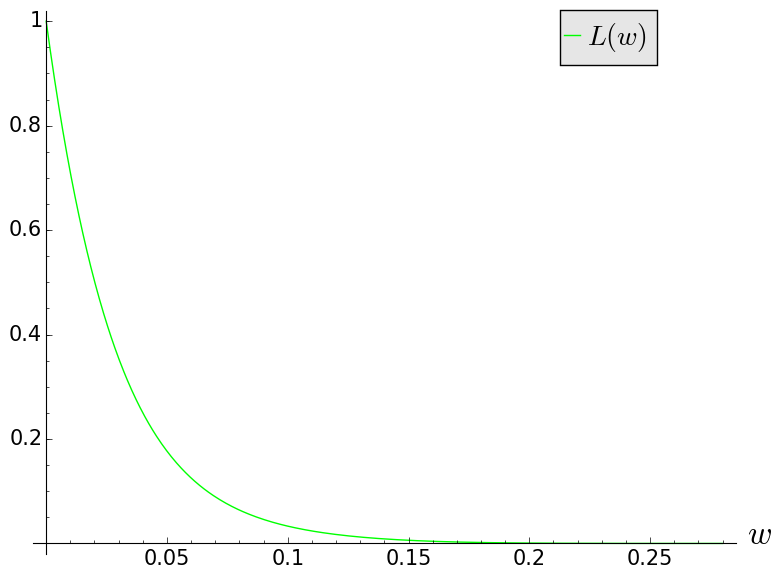
\includegraphics[width=0.4\linewidth]{plots/ch1_16_L.png}
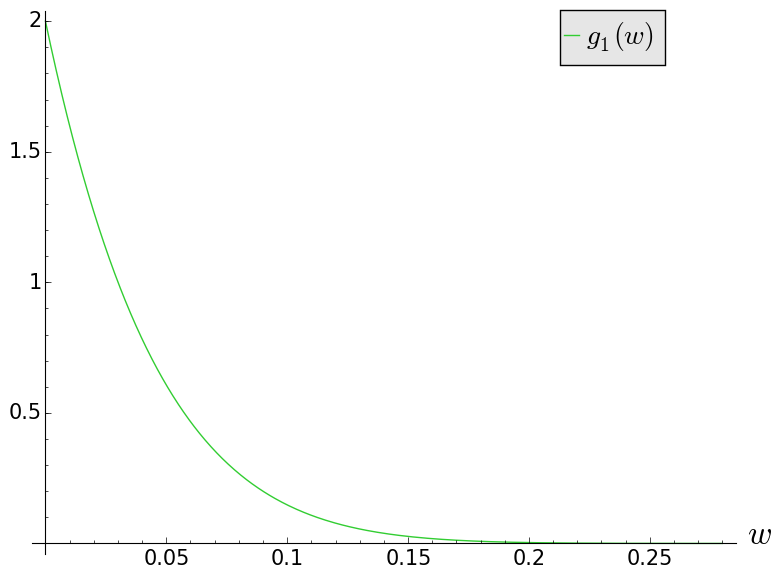
\includegraphics[width=0.4\linewidth]{plots/ch1_17_g_1.png}
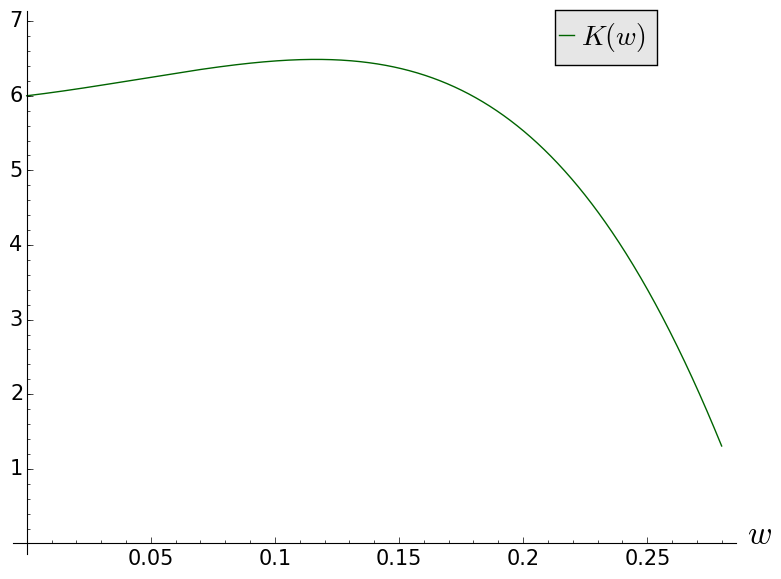
\includegraphics[width=0.4\linewidth]{plots/ch1_18_K.png}
\vspace{0.5cm}			
			
As we see in the figures they indeed are. This has been also checked with Sturm algorithm and numerically with Sage. Thus, $(\spadesuit)$ holds and the result is proved. \qed
\end{subsection}
\end{section}
\end{chapter}

\begin{chapter}{A short proof for the open quadrant $\Qu$ problem}
\begin{section}{Introduction}
Hello world...


%Ejemplo de como introducir texto con TikZ, con una rejilla de ayuda
\begin{figure}[h]
%\centering
\begin{tikzpicture}
\node[anchor=south west,inner sep=0] (img)at (0,0) {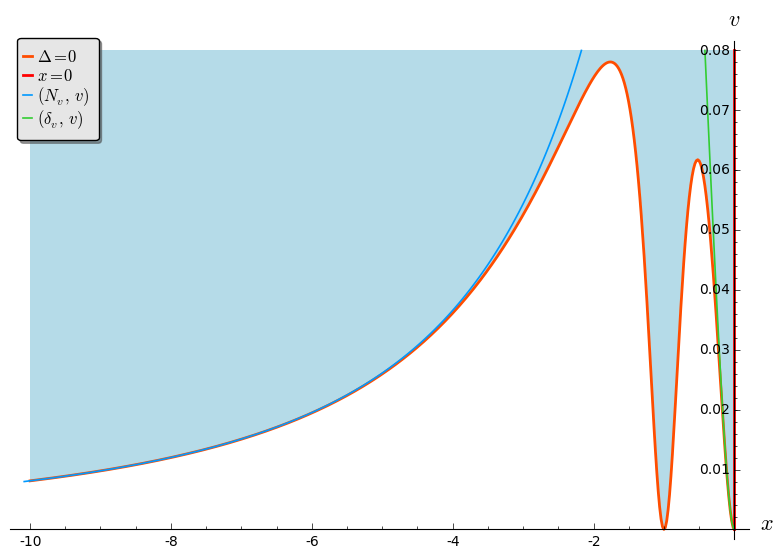
\includegraphics[width=\textwidth]{plots/ch1_15_nice_plot.png}};
\foreach \xx in {0,1,2,...,9}{
\draw[dashed] ($(img.north west)!0.\xx!(img.north east)$)node[above]{0.\xx} --  ($(img.south west)!0.\xx!(img.south east)$);
\draw[dashed] ($(img.south east)!0.\xx!(img.north east)$)node[right]{0.\xx} --  ($(img.south west)!0.\xx!(img.north west)$);
}
\path ($(img.north west)!0.1!(img.north east)$)|-coordinate(c1)($(img.south east)!0.3!(img.north east)$);% c1: first corner
\path ($(img.north west)!0.82!(img.north east)$)|-coordinate(c2)($(img.south east)!0.77!(img.north east)$);   %c2 : second corner
\draw[red,ultra thick,rounded corners] (c1)         rectangle (c2);
\draw (c1) node {\huge{$\mathscr{A}$}};
\draw (c2) node[below] {\huge{$\mathscr{B}$}};
\end{tikzpicture}
\caption{M1} \label{fig:M1}
\end{figure}

\end{section}
\end{chapter}

\appendix
\begin{chapter}{Auxiliary definitions and results}

\begin{definition}\label{realCField}
	A \em real closed field \em is an ordered field $R$ such that $R(\sqrt{-1})$ is an algebraically closed field. There exist many characterizations of real closed fields. A very enlightening is the following one: $R$ is a real closed field if it is an ordered field that shares with the field $\R$ of real numbers its properties of the first-order language of ordered fields. 
\end{definition}

Indeed, \hyperref[tarskiSeidenberg]{Tarski-Seidenberg Theorem} admits a useful formulation in model theory that explains accurately our last sentence.

\begin{theorem}[\em Transfer Principle\em]\label{TP} \em Let ${\mathcal L}(R)$ be the first-order language of ordered fields with parameters in the real closed field $R$ and let $\Phi$ be a formula of ${\mathcal L}(R)$. Then, there exists a quantifier-free formula $\Psi$ of ${\mathcal L}(R)$ with the same free variables $x_1,\dots,x_n$ as $\Phi$ such that, for every real closed field extension $K$ of $R$ and every $x\in K^n$, the sentence $\Phi(x)$ holds true if and only if $\Psi(x)$ holds true.\em

\end{theorem}


\begin{definitions}\label{semialgSet} (i) Let $R$ be a real closed field. A subset $S\subset R^n$ is \em semialgebraic \em if it is defined as a finite union of sets defined by a conjunction of polynomial equalities and inequalities: 
	\begin{equation*}
	\left\{
	\begin{aligned}
		P_1(x_1,\, .\,&.\,.\, , x_n) = 0\\
		&\vdots\\
		P_r(x_1, .\,&.\,.\, , x_n) = 0 \\
		Q_1(x_1, .\,&.\,.\, , x_n) > 0 \\
		&\vdots\\
		Q_{\ell}(x_1, .\,&.\,.\, , x_n) > 0 \\
	\end{aligned}
	\right.
	\end{equation*}
It is easily seen that finite unions and intersections of semialgebraic sets are semialgebraic sets too. In addition, the complementary set of a semialgebraic set is also a semialgebraic set. The easy proof of these facts can be studied in \cite{bcr}, Ch.2.
	
	
(ii) A map $f:S\to T$ between semialgebraic subsets $S\subset R^n$ and $T\subset R^m$ is \em semialgebraic \em if its graph is a semialgebraic subset of $R^{m+n}$.  \end{definitions}


(iii) A \em semialgebraic homeomorphism \em between two semialgebraic subsets $S\subset R^n$ and $T\subset R^m$ is a continuous and bijective semialgebraic map $f:S\to T$. It is easily seen that in such a case its inverse $f^{-1}:T\to S$ is also semialgebraic.


\begin{definition}[Zariski topology]\label{zariski} (i) Let $K$ be a field. A subset $X\subset K^n$ is \em algebraic \em if it is the set of common zeros of a finite family of polynomials $f_1,\dots,f_m\in K[x_1,\dots, x_n]$. 

(ii) The \em Zariski topology \em of an algebraic set $X\subset K^n$ is the topology whose closed sets are the algebraic subsets of $K^n$ contained in $X$. It is indeed a topology, that is, the arbitrary intersection of algebraic sets is also an algebraic set as an straightforward consequence of Hilbert's basis theorem.

(iii) An algebraic subset $X\subset K^n$ is said to be \em reducible \em if there exist algebraic subsets $Y\subsetneq X$ and  $Z\subsetneq X$ such that $X=Y\cup Z$. If $X$ is not reducible it is said to be  \em irreducible. \em 
\end{definition}

\begin{definition}\label{pureDim} (i) Let $S\subset\R^n$ be a semialgebraic set and $p\in S$. The \em local dimension of $S$ at $p$, \em denoted $\dim(S_p)$, is the largest non-negative integer $d$ such that for every open ball $B$ centered at $p$ the intersection $S\cap B$ contains a semialgebraic subset semialgebraically homeomorphic to the cube $[0,1]^d$.

	It is said that $S$ is \em pure dimensional \em if $\dim(S_p)=\dim(S_q)$ for every pair of points $p,q\in S$.
\end{definition}

\begin{definitions}\label{properMap}
	  (i) A continuous map $f:X\to Y$ between topological spaces $X$ and $Y$ is said to be \em proper \em if $f^{-1}(K)$ is a compact subspace of $X$ for every compact subspace $K$ of $Y$. 
	  
	  (ii) A semialgebraic map $f:S\to T$ between semialgebraic sets $S\subset R^n$ and $T\subset R^m$ is said to be \em semialgebraically proper \em if $f^{-1}(K)$ is bounded and closed in $S$ for every bounded and closed in $T$ subset $K$ of $T$.  
\end{definitions}

\begin{definition}\label{dominant}
	A polynomial map $f:X\to Y$ between algebraic sets $X$ and $Y$ is said to be \em dominant \em if its image $f(X)$ is a dense subset of $Y$ in its Zariski topology. 
\end{definition}

\begin{definitions}\label{curveGerms}
	(i) A function $f:U\to\R$ defined in an open semialgebraic subset $U\subset\R^n$ is a \em Nash function \em if it is analytic and semialgebraic. A map $f:=(f_1,\dots,f_m):U\to\R^m$ is a \em Nash map \em if each coordinate $f_i:U\to\R$ is a Nash function. 
	
	(ii) Let $\Gamma\subset\R^n$ be an algebraic curve and $p\in\Gamma$. For every small enough $\varepsilon>0$ the intersection $B_{\varepsilon}\cap\Gamma\setminus\{a\}$, % Aqui no sería p en vez de a?
where $B_{\varepsilon}\subset\R^n$ is the open ball of radius $\varepsilon$ centered at the point $p$, has finitely many connected components $C_1,\dots,C_k$. Each $C_i$ is semialgebraically homeomorphic to the interval $(0,1]$ and in fact for $i=1,\dots,k$ there exists a Nash homeomorphism  $f_i:[0,1]\to C_i\cup\{p\}$, with $f_i(0)=p$.

Indeed, this result is a particular case of the local conic structure theorem of semialgebraic sets. 
	
Observe that, by its very definition, it makes sense to define the germs $C_{i,p}$ of $C_i$ at the point $p$ for $i=1,\dots,k$ as they are independent of the radius $\varepsilon$. These germs  $C_{i,p}$ are called the \em germ Nash half-banches \em of the curve $\Gamma$ centered at $p$. For more details see \cite[IX.5.2]{bcr}. 
\end{definitions}

\begin{definition} \label{puiseux} It is proved in \cite[pp. 98-102]{w} that given an algebraically closed field $K$ and an indeterminate ${\tt t}$ over $K$, the field $K\left(\set{{\tt t}^*}\right)$ of \em Puiseux series \em with coefficients in $K$ is algebraically closed. As it is an algebraic extension of the field $K\left({\tt t}\right)$ of rational functions over $K$, the field $K\left(\set{{\tt t}^*}\right)$ is an algebraic closure of the field $F({\tt t})$ for every subfield $F$ of $K$ such that the field extension $K|F$ is algebraic. In particular, for $F:=\R$ it follows that $\C\left(\set{{\tt t}^*}\right)$ is an algebraic closure of $\R({\tt t})$.
\end{definition}

Sturm method is used to obtain the number of different real roots of a polynomial in a given interval.

\begin{definitions}\label{sturmSeq} (i) Let $R$ be a real closed field and $f,g\in\R[x]$ be polynomials. A  \emph{Sturm sequence} (or \emph{Sturm chain}) is a finite sequence of polynomials $(f_0, f_1, \dots, f_k)$ where 
\begin{equation*}
\begin{aligned}
f_0 &:= f\\
f_1 &:= f'g\\
& \dots\\
f_i &:= f_{i-1}q_i - f_{i-2}, \text{ with } q_{i}\in R[x] \text{ and } \text{deg}(f_{i}) < \text{deg}(f_{i-1}) \text{ for } i = 2, \dots, k.\\
\end{aligned}
\end{equation*}
	Then, by Euclid's Algorithm, there is an integer $k$ verifying $f_k = \text{gcd}(f, f'g)$.
	
(ii) Given a sequence $(a_0, a_1, \dots, a_k)$ of elements of $R$ with $a_0 \ne 0$, we define the \emph{number of sign changes in the sequence} $(a_0, \dots, a_k)$ as follows: count one sign change every time $a_ia_{\ell} < 0$, with 
\begin{equation*}
\begin{aligned}
&\ell = i + 1 \text{, or }\\
&\ell > i + 1 \text{ and } a_j = 0 \text{ for every } j \text{ verifying  } i < j < \ell.\\ 
\end{aligned}
\end{equation*}

(iii) If $a \in R$ is not a root of $f$ and $(f_0, \dots, f_k)$ is the Sturm sequence of $f$ and $g$, we define $v(f, g, a)$ to be the number of sign changes in $(f_0(a), \dots, f_k(a))$.
\end{definitions}
\begin{proposition}[Sturm's Theorem]\label{sturm} 
Let $R$ be a real closed field and $f \in R[x]$. Let $a, b \in R$ be such that $a < b$ and neither $a$ nor $b$ are roots of $f$. Then the number of roots of $f$ in the interval $(a, b)$ is equal to $v(f, 1, a) - v(f, 1, b)$.

\em The proof of this proposition can be studied in \cite[1.2.10]{bcr}. \em
\end{proposition}


\end{chapter}

\begin{thebibliography}{10}

\bibitem[ABR]{abr} C. Andradas, L. Br\"ocker, J.M. Ruiz: Constructible 
sets in real geometry. \em Ergeb. Math. \em{\bf 33}. Berlin, Heidelberg, 
New York: Springer Verlag, (1996).

\bibitem[BCR]{bcr} J. Bochnak, M. Coste, M.-F. Roy: G\'eom\'etrie
alg\'ebrique r\'eelle. \em Ergeb. Math. \em {\bf 12}, Springer-Verlag,
Berlin, Heidelberg, New York (1987).

\bibitem[FG]{fg} J.F. Fernando, J.M. Gamboa: Polynomial images of $R^n$.
\textit{Journal of Pure and Applied Algebra}, {\bf 179}, (2003), no. 3, 241-254.

\bibitem[FGU]{fgu} J.F. Fernando, J.M. Gamboa, C. Ueno: The open quadrant problem:
A topological proof. \textit{Preprint} (2015), 13 pages.

\bibitem[FU]{fu} J.F. Fernando, C. Ueno: A short proof for the open quadrant problem.
\textit{Preprint RAAG} (2014, submitted to MEGA 2015), 8 pages.

\bibitem[G]{g} J.M. Gamboa: Reelle algebraische Geometrie, June,
$10^{\text{th}}-16^{\text{th}}$ (1990), \textit{Oberwolfach}.

\bibitem[W]{w} R.J. Walker: \em Algebraic curves. \em Berlin, Heidelberg, 
New York: Springer Verlag, (1978).



\end{thebibliography}


\end{document}
